%%%%%%%%%%%%%%%%%%%% author.tex 
%%%%%%%%%%%%%%%%%%%%%%%%%%%%%%%%%%%
%
% sample root file for your "contribution" to a proceedings volume
%
% Use this file as a template for your own input.
%
%%%%%%%%%%%%%%%% Springer 
%%%%%%%%%%%%%%%%%%%%%%%%%%%%%%%%%%


\documentclass{svproc}
%
% RECOMMENDED 
%%%%%%%%%%%%%%%%%%%%%%%%%%%%%%%%%%%%%%%%%%%%%%%%
%%%
%
\usepackage{graphicx}
\usepackage{marvosym}
\usepackage{amsmath}
\usepackage{amssymb}
\usepackage{cite}

%\usepackage[russian]{babel}

% to typeset URLs, URIs, and DOIs
\usepackage{url}
\usepackage{hyperref}
\def\UrlFont{\rmfamily}

\def\orcidID#1{\unskip$^{[#1]}$}
\def\letter{$^{\textrm{(\Letter)}}$}

\begin{document}
\mainmatter              % start of a contribution
%
\title{Adaptive global optimization using graphics accelerators\thanks{This study was supported by the Russian Science Foundation, project No.\,16-11-10150.}
}
%
\titlerunning{Adaptive global optimization}  % abbreviated title (for running head)
%                                     also used for the TOC unless
%                                     \toctitle is used
%
\author{Konstantin Barkalov%\orcidID{0000-0001-5273-2471} 
\and Ilya Lebedev\letter%\orcidID{0000-0002-8736-0652}
}

%
\authorrunning{Konstantin Barkalov \and Ilya Lebedev} % abbreviated author list (for running head)
%
%%%% list of authors for the TOC (use if author list has to be modified)
\tocauthor{Konstantin Barkalov and Ilya Lebedev}
%
\institute{Lobachevsky State University of Nizhni Novgorod, Russia  \\
	\email{konstantin.barkalov@itmm.unn.ru},
	\email{ilya.lebedev@itmm.unn.ru}
}
	
\maketitle              % typeset the title of the contribution

\begin{abstract}

Problems of multidimensional multiextremal optimization and numerical methods for their solution are considered. The general assumption is made about the function being optimized: it satisfies the Lipschitz condition with an a priori unknown constant. Many approaches to solving problems of this class are based on reducing the dimension of the problem; i.e. addressing a multidimensional problem by solving a family of problems with lower dimension. In this work, an adaptive dimensionality reduction scheme is investigated, and its implementation using graphic accelerators is proposed. Numerical experiments on several hundred test problems were carried out, and they confirmed acceleration in the developed GPU version of the algorithm.


\keywords{Global optimization $\cdot$ Multiextremal functions $\cdot$ Reduction of dimensionality $\cdot$ Peano space-filling curves $\cdot$ Recursive optimization $\cdot$ Graphics accelerators }
\end{abstract}

\section{Introduction}

A promising direction in the field of parallel global optimization (which, indeed, is true in many areas related to the software implementation of time-consuming algorithms) is the use of graphics processing units (GPUs). In the past decade, graphics accelerators have rapidly increased performance to meet the ever-growing demands of graphics application developers. Additionally, in the past few years some principles for developing graphics hardware have changed, and as a result it has become more programmable. Today, a graphics accelerator is a flexibly programmable, massive parallel processor with high performance, which is in demand for solving a range of computationally time-consuming problems \cite{Hwu2011}.

However, the potential for graphics accelerators to solve global optimization problems has not yet been fully realized. Using  GPUs, they basically parallelize nature-inspired optimization algorithms, which are somehow based on the idea of random search (see, for example, \cite{Ferreiro2013,Garcia2014,Langdon2011}). By virtue of their stochastic nature, algorithms of this type guarantee convergence to the global minimum only in the sense of probability, which differentiates them unfavorably from deterministic methods.

With regard to many deterministic algorithms of Lipschitzian global optimization with guaranteed convergence, parallel variants have been proposed \cite{Evtushenko2009,He2008,Paulavicius2011}. However, these versions of algorithms are parallelized on CPU using shared and/or distributed memory; presently, no GPU implementations have been made. For example, \cite{Paulavicius2011} describes parallelization of an algorithm based on the ideas of the branch and boundary method using MPI and OpenMP.

Within the framework of this research, we consider the problems of capturing the optimum, which are characterized by a lengthy period for calculating the values of objective function in comparison with the time needed for processing them. For example, objective function can be specified using systems of linear algebraic equations, systems of ordinary differential equations, etc. Currently, graphics accelerators can be used to solve problems of this type. Moreover, an accelerator can solve several such problems at once \cite{Kindratenko2014}; i.e., using GPU, one can calculate multiple function values simultaneously.

Thus, calculating the optimization criterion can be implemented on GPU, and the role of the optimization algorithm (running on CPU) consists in the effective selection of points for conducting parallel trials. This scheme of working with the accelerator is fully consistent with the work of the parallel global search algorithm developed at the Lobachevsky State University of Nizhni Novgorod and presented in a series of publications \cite{Barkalov2014,Barkalov2020,Barkalov2019,Grishagin2016,Grishagin2015,Grishagin2018,globalizerSystem}.


\section{Multidimensional parallel global search algorithm}
Consider the problem of finding the global minimum of the \(N\)-dimensional function \(\varphi(y)\) in the hyperinterval  \(D=\{y\in R^N:a_i\leqslant x_i\leqslant{b_i}, 1\leqslant{i}\leqslant{N}\}\).  We will assume that the function satisfies the Lipschitz condition with an a priori unknown constant \(L\).
\begin{equation}
\label{task}
\varphi(y^*)=\min\{\varphi(y):y\in D\},
\end{equation}
\begin{equation}
\label{lip}
|\varphi(y_1)-\varphi(y_2)|\leqslant L\Vert y_1-y_2\Vert,y_1,y_2\in D,0<L<\infty.
\end{equation}

In this paper, we will use an approach based on the idea of reducing dimensionality using the Peano space-filling curve \(y(x)\), which continuously and unambiguously maps a segment of the real axis \([0,1]\) onto an \(n\)-dimensional cube
\begin{equation}
\label{cube}
\lbrace y\in R^N:-2^{-1}\leqslant y_i\leqslant 2^{-1},1\leqslant i\leqslant N\rbrace=\{y(x):0\leqslant x\leqslant 1\}.
\end{equation}

The questions of numerical construction of approximations to Piano curve (evolvents) and the corresponding theory are discussed in detail in \cite{Sergeyev2013,Strongin2000}. Using evolvents \(y(x)\) reduces the multidimensional problem (\ref{task}) to a one-dimensional problem
\begin{displaymath}
\label{oneDimTask}
\varphi(y^*)=\varphi(y(x^*))=\min\{\varphi(y(x)):x\in [0,1]\}.
\end{displaymath}

An important property is that the relative differences of the function remain limited: if the function \(\varphi(y)\) in the region \(D\) satisfies the Lipschitz condition, then the function \(\varphi(y(x))\) in the interval \([0,1]\) will satisfy a uniform H{\"o}lder condition
\begin{displaymath}
\label{holder}
|\varphi(y(x_1))-\varphi(y(x_2))|\leqslant H{|x_1-x_2|}^{\frac{1}{N}}, x_1,x_2\in[0,1],
\end{displaymath}
where the H{\"o}lder constant \(H\) is related to the Lipschitz constant \(L\) by the ratio $ H=2L\sqrt{N+3}$. 
Therefore, without limiting generality, we can consider minimizing the one-dimensional function \(f(x)=\varphi(y(x)), x\in[0,1]\), which satisfies the H{\"o}lder condition.

The algorithm for solving this problem (Global Search Algorithm, GSA) involves constructing a sequence of points \(x_k\), in which the values of objective function \(z_k = f(x_k)\) are calculated. We will call the process of computing the value of a function at a single point a trial. Assume that we have \(p\geqslant 1\) computational elements at our disposal and \(p\) trials which are performed simultaneously (synchronously) within a single iteration of the method. Let \(k(n)\) denote the total number of trials performed after \(n\) parallel iterations.

At the first iteration of the method, the trial is carried out at an arbitrary internal point \(x^1\) of the interval \([0,1]\). Let \(n>1\) iterations of the method be performed, during which trials were carried out at \(k = k(n)\) points \(x^i, 1\leqslant i\leqslant k\). Then the trial points  \(x^{k+1},\dotsc,x^{k+p}\) of the next \((n+1)\)-th iteration are determined in accordance with the following rules.

Step 1. Renumber the points of the set \(X_k=\{x^1,\dotsc,x^k\}\cup\{0\}\cup\{1\}\), which includes the boundary points of the interval \([0,1]\), as well as the points of the previous trials, with the lower indices in the order of their increasing coordinate values, i.e.
\begin{displaymath}
0=x_0<x_1<\dotsc<x_{k+1}=1.
\end{displaymath}

Step 2. Assuming \(z_i=f(y(x_i)),1\leqslant i\leqslant k\), calculate the values
\begin{displaymath}
\label{step2}
\mu=\max_{1\leqslant i\leqslant k}\dfrac{|z_i-z_{i-1}|}{\Delta_i}, \;
\begin{matrix}
    M = 
    \left\{
    \begin{matrix}
    r\mu,\mu>0, \\
    1,\mu=0,
    \end{matrix} \right.
    \end{matrix}
\end{displaymath}
where \(r > 1\) is the specified parameter of the method, and \(\Delta_i=(x_i-x_{i-1})^\frac{1}{N}\). 

Step 3. For each interval \((x_{i-1},x_i),1\leqslant i\leqslant k+1\), calculate the characteristic in accordance with the formulas 
\begin{displaymath}
\label{step3_1}
R(1)=2\Delta_1-4\dfrac{z_1}{M}, \; R(k+1)=2\Delta_{k+1}-4\dfrac{z_k}{M},
\end{displaymath}
\begin{displaymath}
\label{step3_2}
R(i)=\Delta_i+\dfrac{(z_i-z_{i-1})^2}{M^2\Delta_i}-2\dfrac{z_i+z_{i-1}}{M},1<i<k+1.
\end{displaymath}

Step 4. The characteristics \(R(i),1\leqslant i\leqslant k+1\), arrange in descending order 
\begin{displaymath}
\label{step4}
R(t_1)\geqslant R(t_2)\geqslant \dots \geqslant R(t_{k})\geqslant R(t_{k+1})
\end{displaymath}
and select \(p\) of the largest characteristics with interval numbers \(t_j,1\leqslant j\leqslant p\).

Step 5. Carry out new trials at the points \(x_{k+j},1\leqslant j\leqslant p\), calculated using the formulas
\begin{displaymath}
x_{k+j}=\dfrac{x_{t_j}+x_{t_j-1}}{2},\; t_j=1, \; t_j=k+1
\end{displaymath}
\begin{displaymath}
\label{step5}
{{x}^{k+1}}=\frac{{{x}_{{{t}_{j}}}}+{{x}_{{{t}_{j}}-1}}}{2}-\text{sign}({{z}_{{{t}_{j}}}}-{{z}_{{{t}_{j}}-1}})\frac{1}{2r}{{\left[ \frac{|{{z}_{{{t}_{j}}}}-{{z}_{{{t}_{j}}-1}}|}{\mu } \right]}^{N}}, 1<{{t}_{j}}<k+1.
\end{displaymath}

The algorithm stops working if the condition \(\Delta_{t_j}\leqslant \varepsilon\)  is satisfied for at least one number \(t_j,1\leqslant j\leqslant p\); here \(\varepsilon>0\)  is the specified accuracy. As an estimate of the globally optimal solution to the problem (\ref{task}), the values are selected 
\begin{displaymath}
f_{k}^{*}=\underset{1\le i\le k}{\mathop{\min }}\,f({{x}^{i}}),   x_{k}^{*}=\arg \; \underset{1\le i\le k}{\mathop{\min }}\,f({{x}^{i}}).
\end{displaymath}
For the rationale in using this method of organizing parallel computing see \cite{Strongin2000}. 
%Modifications that account for the presence of inequality constraints in the problem, as well as information about the derivative of the objective function, are presented in \cite{Ref12} – \cite{Ref14}.

\section{Dimensionality reduction schemes in global optimization problems}

\subsection{Dimensionality reduction using multiple mappings}

Reducing multidimensional problems to one-dimensional ones through the use of evolvents has important properties such as continuity and preserving uniform bounding of function differences with limited argument variation. However, some information about the proximity of points in multidimensional space is lost, since the point \(x\in [0,1]\) has only left and right neighbors, and the corresponding point \(y(x) \in R^N\) has neighbors in \(2^N\) directions. As a result, when using evolvents, the images \(y' , y''\) that are close in \(N\)-dimensional space can correspond to rather distant preimages \(x' , x''\) on the interval \([0,1]\). This property leads to redundant calculations, because several limit points \(x' , x''\) of the test sequence generated by the method on the segment \([0,1]\), can correspond to a single limit point \(y\) in \(N\)-dimensional space.

A possible way to overcome this disadvantage is to use a set of evolvents (multiple mappings)
\begin{displaymath}
\label{eq:142}
Y_L(x)=\left\{y^0(x),\ y^1(x),...,\ y^L(x)\right\}
\end{displaymath}
instead of using a single Peano curve \(y(x)\) (see \cite{Strongin1992,Strongin2000}). For example, each Peano curve \(y^i(x)\) from \(Y_L(x)\) can be obtained as a result of some shifting \(y(x)\) along the main diagonal of the hyperinterval \(D\). Another way is to rotate the evolvent \(y(x)\) around the origin. The set of evolvents that have been constructed allows us to obtain for any close images \(y', y''\) close preimages \(x', x''\) for some mapping \(y^i(x)\).

Using a set of mappings leads to the formation of a corresponding set of one-dimensional multiextremal problems
\begin{displaymath}
\label{6_problem_l}
\min{\left\{\varphi(y^l(x)):x\in [0,1], \;  \right\}}, \ 0 \leqslant l \leqslant L.
\end{displaymath}
Each problem from this set can be solved independently, and any calculated value \(z= \varphi(y')\), \(y'=y^i(x')\) of the function \(\varphi(y)\) in the \(i\)-th problem can be interpreted as calculating the value \(z= \varphi(y')\), \(y'=y^s(x'')\) for any other \(s\)-th problem without repeated labor-intensive calculations of the function \(\varphi(y)\). Such informational unity makes it possible to solve the entire set of problems in a parallel fashion. This approach was discussed in detail in \cite{Barkalov2019}.


\subsection{Recursive dimensionality reduction scheme}

The recursive optimization scheme is based on the well-known relation
\begin{equation}
\label{nestedScheme}
\min{\varphi(y):y\in D}=\min_{a_1\leqslant y_1\leqslant b_1}\min_{a_2\leqslant y_2\leqslant b_2}\dots\min_{a_1\leqslant y_N\leqslant b_N}\varphi(y),
\end{equation}
which allows one to replace the solution of the multidimensional problem (\ref{task}) with the solution of a family of one-dimensional subproblems recursively related to each other.
Let's introduce a set of functions

\begin{equation}
\label{phiN}
\varphi_N(y_1,\dots,y_N)=\varphi(y_1,\dots,y_N),
\end{equation}
\begin{equation}
\label{phiI_}
\varphi_i(y_1,\dots,y_i)=\min_{a_{i+1}\leqslant y_{i+1} \leqslant b_{i+1}}\varphi_{i+1}(y_1,\dots,y_i,y_{i+1}),1\leqslant i\leqslant N-1.
\end{equation}

Then, in accordance with the relation (\ref{nestedScheme}), the solution of the original problem (\ref{task}) is reduced to the solution of a one-dimensional problem
\begin{equation}
\label{phiFirst}
\varphi_1(y_1^*)=\min\{\varphi_1(y_1),y_1\in [a,b]\}.
\end{equation}

However, each calculation of the value of the one-dimensional function  \(\varphi_1(y_1)\) at some fixed point corresponds to the solution of a one-dimensional minimization problem 
\begin{displaymath}
\label{phi2}
\varphi_2(y_1,y_2^*)=\min\{\varphi(y_1,y_2):y_2\in [a_2,b_2]\}.
\end{displaymath}
And so on, until the calculation   according to (\ref{phiN}). 

For the recursive scheme described above, a generalization (\textit{block recursive scheme}) is proposed that combines the use of evolvents and a recursive scheme in order to efficiently parallelize computations.

Consider the vector $y$ as a vector of block variables
\begin{displaymath}
y=(y_1,\dots,y_N)=(u_1,u_2,\dots,u_M),
\end{displaymath}
where the \(i\)-th block variable \(u_i\) is a vector of sequentially taken components of the vector \(y\), i.e. $u_1=(y_1,y_2,\dots,y_{N_1})$,$u_2=(y_{N_1+1},y_{N_1+2},\dots,y_{N_1+N_2})$,$\dots,u_M=(y_{N-N_M+1},y_{N-N_M+2},\dots,y_N)$, while \(N_1+N_2+\dots+N_M=N\).

Using new variables, the main relation of the multistep scheme (\ref{nestedScheme}) can be rewritten as
\begin{equation}
\label{blockNested}
\min_{y\in D} \varphi(y)=\min_{u_1\in D_1}\min_{u_2\in D_2}\dots\min_{u_M\in D_M}\varphi(y),
\end{equation}
where the subdomains  \(D_i,1\leqslant i\leqslant M\), are projections of the original search domain \(D\) onto the subspaces corresponding to the variables \(u_1,1\leqslant i\leqslant M\).

The formulas that determine the method for solving problem (\ref{task}) based on relations (\ref{blockNested}) generally coincide with the recursive scheme (\ref{phiN})--(\ref{phiFirst}). One need only replace the original variables  \(y_i,1\leqslant i\leqslant N\), with block variables  \(u_1,1\leqslant i\leqslant M\). 
In this case, the fundamental difference from the original scheme is the fact that the block scheme has nested subproblems
\begin{equation}
\label{subTasks}
\varphi_i(u_1,\dots,u_i)=\min_{u_{i+1}\in D_{i+1}}\varphi_{i+1}(u_1,\dots,u_i,u_{i+1}),1\leqslant i\leqslant M-1,
\end{equation}
which are multidimensional, and to solve them, a method of reducing dimensionality based on Peano curves can be applied.

\subsection{Adaptive dimensionality reduction scheme}

The solution to the resulting set of subproblems (\ref{subTasks}) can be organized in various ways.
The obvious method (elaborated in detail in \cite{Grishagin2015} for the nested optimization scheme and in \cite{Barkalov2014} for the block nested optimization scheme) is based on solving subproblems in accordance with the recursive order of their generation. However, there is a significant loss of information about the target function.

Another approach is an adaptive scheme in which all subproblems are solved simultaneously, which makes it possible to more fully take into account information about a multidimensional problem and thereby to speed up the process of solving it.
In the case of one-dimensional subproblems, this approach was theoretically substantiated and tested in \cite{Grishagin2016,Grishagin2018}, and in the paper \cite{Barkalov2020} a generalization of the adaptive scheme for multidimensional subproblems was proposed.

The adaptive dimensionality reduction scheme changes the order in which subproblems are solved: they will be solved not one by one (in accordance with their hierarchy in the task tree), but simultaneously, i.e., there will be a number of subproblems that are in the process of being solved. Under the new scheme:	
	\begin{itemize}
		\item to calculate the value of the function of the \(i\)-th level from (\ref{subTasks}), a new \(i+1\)-th level problem is generated in which trials are carried out, after which a new generated problem is included in the set of existing problems to be solved;
		\item the iteration of the global search consists in choosing \(p\) (the most promising) problem from the set of existing problems in which trials are carried out; points for new trials are determined in accordance with the algorithm of subsection 1;
		\item the minimum values of functions from (\ref{subTasks}) are their current estimates based on the accumulated search information.
	\end{itemize}
     
A brief description of the main steps of a block adaptive dimensionality reduction scheme is as follows.
Let the nested subproblems in the form (\ref{subTasks}) be solved using the global search algorithm described in Section 2. Then each subproblem (\ref{subTasks}) can be assigned a numerical value called the characteristic of this problem. As such, we can take the maximum characteristic \(R(t)\) of the intervals formed in this problem. In accordance with the rule for calculating characteristics, the higher the value of the characteristic, the more promising the subproblem is in the continued search for the global minimum of the original problem (\ref{task}). 

Therefore, at each iteration, subproblems with the maximum characteristic are selected for conducting the next trial. The trial either leads to the calculation of the value of the objective function \(\varphi_1(y)\) (if the selected subproblem belonged to the level \(j=M\)), or generates new subproblems according to (\ref{subTasks}) for \(j \geqslant  M-1\). In the latter case, the newly generated problems are added to the current set of problems, their characteristics are calculated, and the process is repeated. The optimization process is completed when the root problem satisfies the condition for stopping the algorithm that solves this problem. Some results pointing in this direction are presented in \cite{Barkalov2020}.


\section{GPU implementation}

\subsection{General scheme}

In relation to global optimization methods, an operation that can be efficiently implemented on GPU is the parallel calculation of many values of the objective function at once. Naturally, this requires implementing a procedure for calculating the value of a function on GPU. Data transfers from CPU to GPU will be minimal: one need only transfer the coordinates of the trial points to GPU, and get back the function values at these points. Functions that determine the processing of trial results in accordance with the algorithm, and require work with large amounts of accumulated search information, can be effectively implemented on CPU.

The general scheme for organizing calculations using GPU is shown in Fig. \ref{fig:GPU_Algorithm}. In accordance with this scheme, steps 1--4 of the parallel global search algorithm are performed on CPU. The coordinates of the $p$ trial points calculated in step 4 of the algorithm are accumulated in the intermediate buffer and then transmitted to GPU. On GPU the function values are calculated at these points, after which the trial results (again through the intermediate buffer) are transferred to CPU.
   
   \begin{figure}[h!]
    \centering
		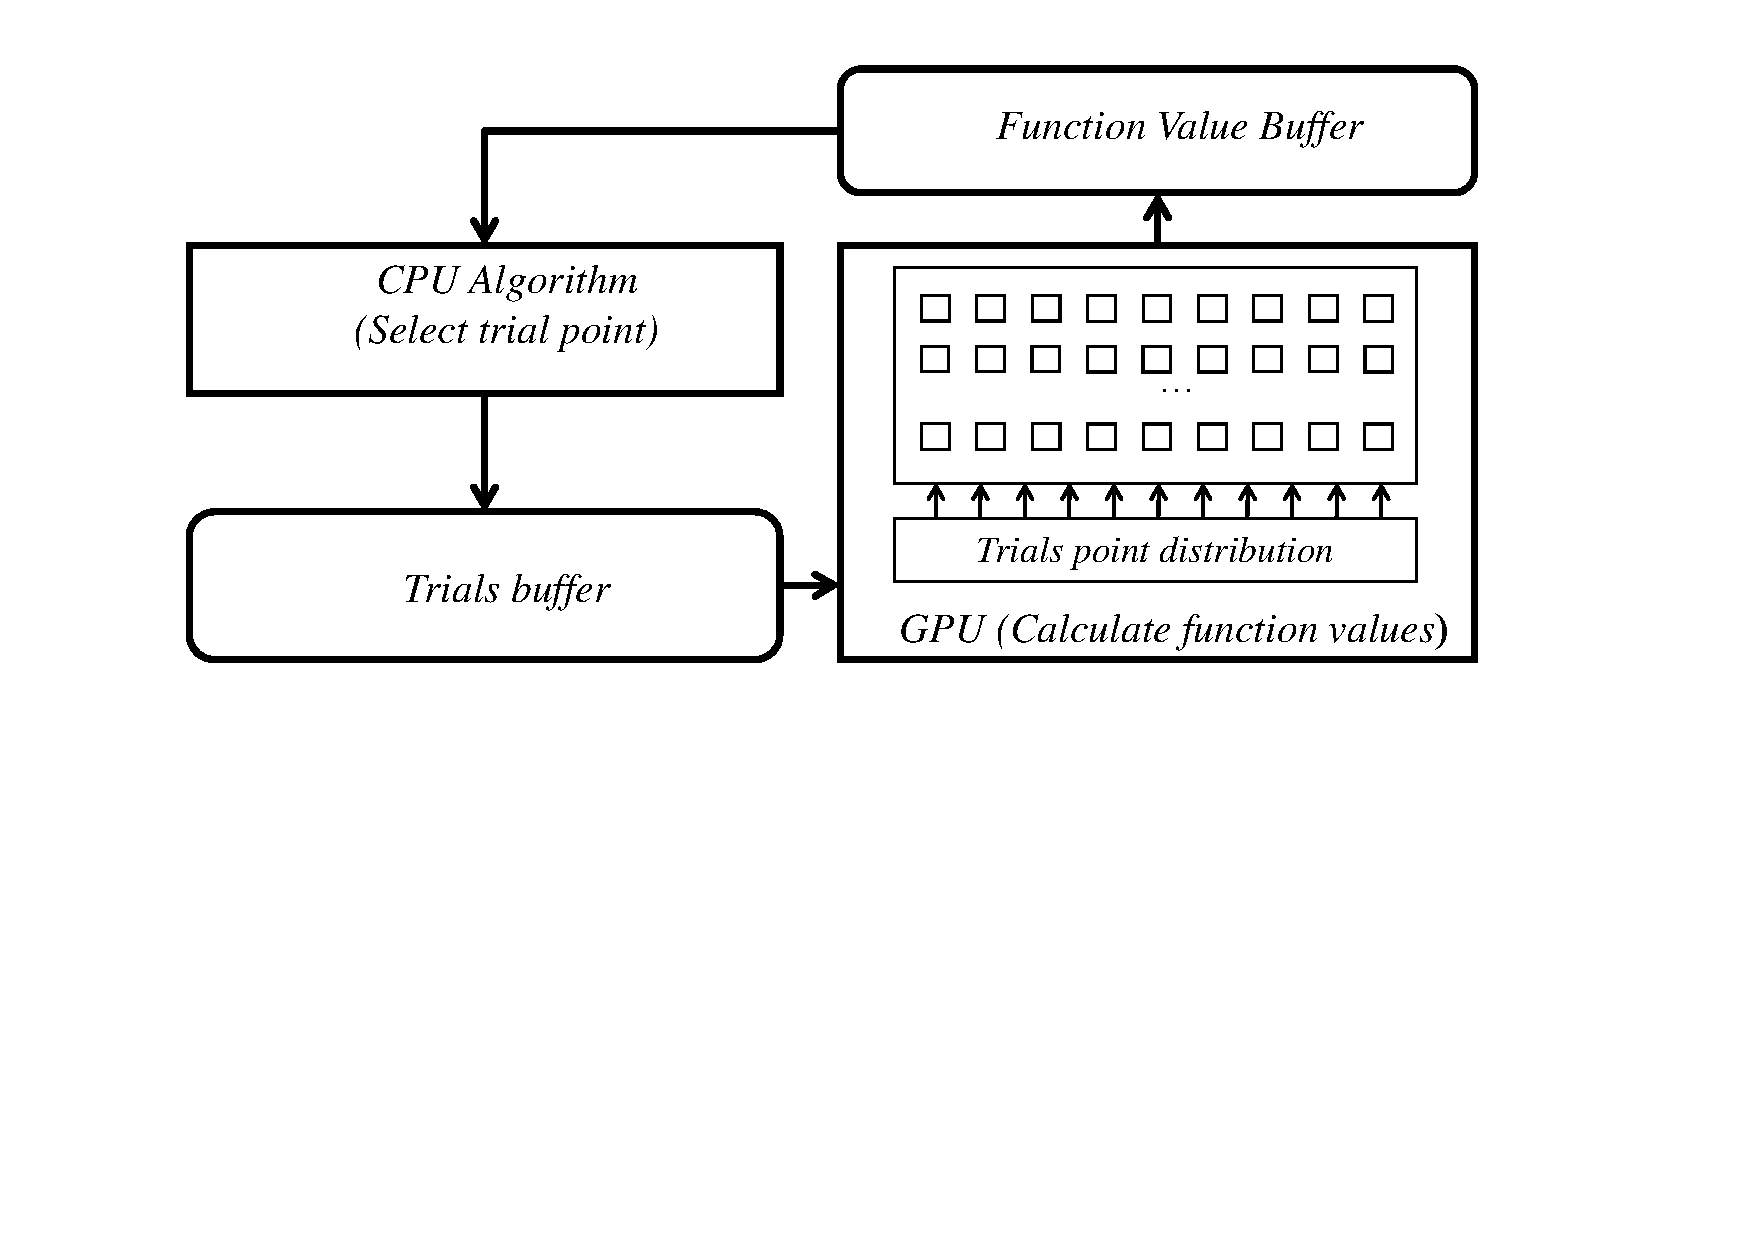
\includegraphics[width=0.9\textwidth]{GPU_Algorithm.pdf}
		\caption{Scheme of information exchanges in the GPU algorithm}\label{fig:GPU_Algorithm}
\end{figure}


\subsection{Organization of parallel computing}

To organize parallel calculations, we will use a set of evolvents and a block adaptive dimensionality reduction scheme. We take a small number of nesting levels, 2 to 3, in which the original large dimensionality problem is divided into 2-3 nested lower dimensional subproblems. We will use multiple evolvents only at the upper level of nesting, corresponding to the u1 variable block. This subproblem will be reduced to a set of one-dimensional problems that will be solved in parallel, each in a separate process. Trial results at point $x$ obtained for the problem solved by a specific processor are interpreted as the trial results in the remaining problems (at the corresponding points \(u^1_1,..., u^s_1\) ).
Then, applying an adaptive scheme to solve the nested subproblems (\ref{subTasks}), we get a parallel algorithm with a wide degree of variability.

\ref{fig:Parallel_Computing} shows the general scheme of organizing calculations using several cluster nodes and several GPUs. In accordance with this scheme, nested subproblems  ${{\varphi }_{i}}({{u}_{1}},...,{{u}_{i}})=\underset{{{u}_{i+1}}\in {{D}_{i+1}}}{\mathop{\min }}\,{{\varphi }_{i+1}}({{u}_{1}},...,{{u}_{i}},{{u}_{i+1}})$  with \(i=1,\ldots ,M-2\) are solved using CPU only. The values of the optimized function are not calculated directly in these subproblems: the calculation the function value  ${{\varphi }_{i}}({{u}_{1}},...,{{u}_{i}})$ is a solution to the minimization problem at the next level.

The subproblem of the last \((M - 1)\)-th level 
\[
{{\varphi }_{M-1}}({{u}_{1}},...,{{u}_{M-1}})=\underset{{{u}_{M}}\in {{D}_{M}}}{\mathop{\min }}\,{{\varphi }_{M}}({{u}_{1}},...,{{u}_{M}})
\]
 differs from all the previous subproblems; it calculates the values of the objective function, since ${{\varphi }_{M}}({{u}_{1}},...,{{u}_{M}})=\varphi ({{y}_{1}},...,{{y}_{N}})$. This subproblem transfers between CPU and GPU.

   \begin{figure}[h!]
    \centering
		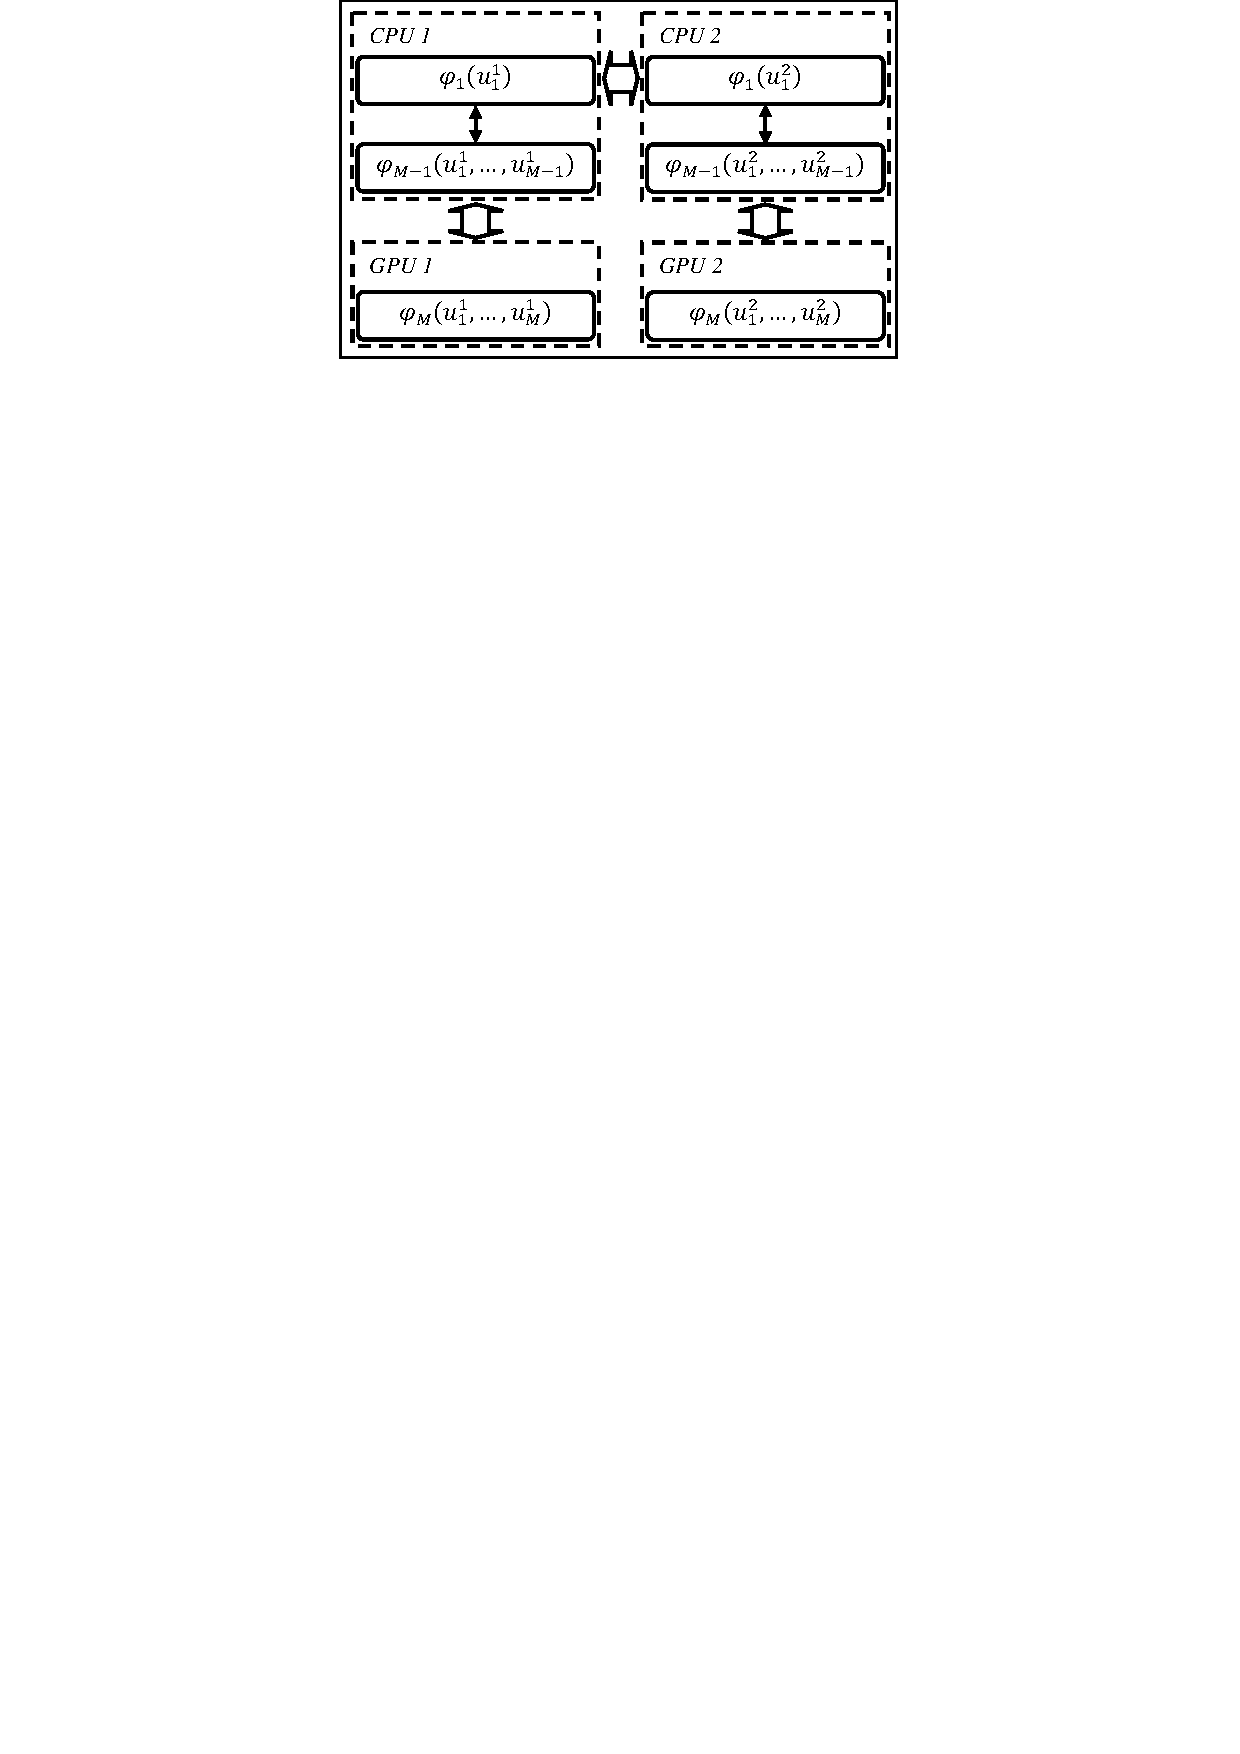
\includegraphics[width=0.7\textwidth]{Parallel_Computing.pdf}
		\caption{Diagram of parallel computing on a cluster}\label{fig:Parallel_Computing}
\end{figure}

\section{Numerical experiments}

The numerical experiments were carried out using the Lomonosov supercomputer (Lomonosov Moscow State University). Each supercomputer node included two quad-core processors Intel Xeon X5570, two NVIDIA Tesla X2070 and 12 Gb RAM. When building the Globalizer system for running on the Lomonosov supercomputer, the GCC 4.3.0 compiler, CUDA 6.5 and Intel MPI 2017 were used.

Note that well-known test problems from the field of multidimensional global optimization are characterized by a short time span for calculating the values of the objective function. Therefore, in order to simulate the computational complexity inherent in applied optimization problems \cite{Modorskii2016}, the calculation of the objective function in all experiments was complicated by additional calculations that do not change the form of the function and the location of its minima (summing the segment of the Taylor series).

In the paper \cite{Gaviano2003} a GKLS generator is described that allows one to generate multiextremal optimization problems with previously known properties: the number of local minima, the size of their regions of attraction, the global minimum point, the value of the function in it, etc.

Below are the results of a numerical comparison of three sequential algorithms -- DIRECT \cite{Jones2009}, DIRECT\textit{l} \cite{Gablonsky2001} and Global Search Algorithm (GSA) from Section 2.  A numerical comparison was carried out on the Simple and Hard function classes of dimension 4 and 5 from \cite{Gaviano2003}. The global minimum $y*$ was considered found if the algorithm generated a trial point $y^k$ in the $\delta$-neighborhood of the global minimum, i.e. $\left\| {{y}^{k}}-{{y}^{*}} \right\| \leqslant \delta $.  Also, the size of the neighborhood was chosen (in accordance with \cite{Sergeyev2006}) as $\delta =\left\| b-a \right\|\sqrt[N]{\Delta }$, here $N$ is the dimension of the problem to be solved , a and b are the boundaries  of the search domain $D$, the parameter  $\Delta ={{10}^{-6}}$ for N=4 and $\Delta ={{10}^{-7}}$ for $N=5$. When using the GSA method for the Simple class, the parameter $r=4.5$ was selected, for the Hard class $r=5.6$; the parameter for constructing the Peano curve was fixed, $m=10$. The maximum number of iterations allowed was $K_{max} = 10^6$.


\begin{table}
	\caption{Average number of iterations $k_{av}$}\label{table:average_iters}
	\center
	\begin{tabular}{ccccc}
		\hline\noalign{\smallskip}
  	 $N$ & Problem class & DIRECT & DIRECT\textit{l} & GSA \\
		\noalign{\smallskip} \hline \noalign{\smallskip}
			4 &	Simple& $>$47282(4) &	18983 &	11953 \\
	      & Hard &	$>$95708(7) &	68754 &	25263 \\
		\noalign{\smallskip}
			5	& Simple &	$>$16057(1) &	16758 &	15920 \\
				& Hard &	$>$217215(16) &	$>$269064(4) & $>$148342(4) \\
		\noalign{\smallskip}\hline
	\end{tabular}
\end{table}


Table \ref{table:average_iters} shows the average number of iterations, $k_{av}$, that the method performed when solving a series of problems from these classes. The symbol \(">"\) reflects a situation where not all problems of the class were solved by any method whatsoever. This means that the algorithm was halted because the maximum allowed number of $K_{max}$ iterations was reached. In this case, the value $K_{max} = 10^6$ was used to calculate the average value of the number of iterations, $k_{av}$, which corresponds to the lower estimate of this average value. The number of unsolved problems is indicated in parentheses.
   
As can be seen from Table \ref{table:average_iters}, the sequential GSA surpasses the DIRECT and DIRECT\textit{l} methods in all classes of problems in terms of the average number of iterations. At the same time, in the 5-Hard class, none of the methods solved all the problems: DIRECT failed to solve 16 problems, DIRECTl and GSA -- 4 problems each.


%\begin{table}
                %\caption{Speedup on CPU}
                %\label{table:average_AS_CPU}
                %\center
                %\begin{tabular}{lccccccccccc}
                               %%\hline\noalign{\smallskip}
																	 %& \multicolumn{5}{c}{ Iteration speedup} & & \multicolumn{5}{c}{ Time speedup}\\
                               %\noalign{\smallskip} \cline{2-6} \cline{8-12}  \\
                                   %& \multicolumn{2}{c}{ $N=4$ } & & \multicolumn{2}{c}{$N=5$} &  & \multicolumn{2}{c}{ $N=4$ } & & \multicolumn{2}{c}{$N=5$} \\
                               %\noalign{\smallskip} \cline{2-3} \cline{5-6}  \cline{8-9} \cline{11-12} \noalign{\smallskip}
                               %& Simple & Hard & & Simple & Hard &  & Simple & Hard & & Simple & Hard  \\
                               %\noalign{\smallskip} \hline \noalign{\smallskip}                               
                               %$p=2$&   3,49 & 2,35 &   & 0,86 & 2,03 &   & 1,71 & 1,17 &   & 0,95 & 0,4 \\
                               %$p=4$&   8,22 & 7,65 &   & 6,74 & 8,56 &   & 2,01 & 1,9  &   & 1,85 & 1,53 \\
                               %\noalign{\smallskip}\hline
                %\end{tabular}
%\end{table}


Let us now evaluate the acceleration achieved using parallel GSA using an adaptive dimensionality reduction scheme based on the number $p$ of cores used.
Table \ref{table:average_MMAS_CPU} shows the speedup of the algorithm that combines multiple evolvents and an adaptive scheme for solving a series of problems on CPU, compared to the sequential launch of the GSA method. Two evolvents and, accordingly, two processes were used; each process used $p$ threads, and calculations were performed on a single cluster node.
% Table \ref{table:average_AS_CPU} shows the speedup obtained when solving a series of problems on the CPU, compared to GSA.
   
\begin{table}
                \caption{Speedup on CPU}
                \label{table:average_MMAS_CPU}
                \center
                \begin{tabular}{lccccccccccc}
                               %\hline\noalign{\smallskip}
																	 & \multicolumn{5}{c}{ Iteration speedup} & & \multicolumn{5}{c}{ Time speedup}\\
                               \noalign{\smallskip} \cline{2-6} \cline{8-12}  \\
                                   & \multicolumn{2}{c}{ $N=4$ } & & \multicolumn{2}{c}{$N=5$} &  & \multicolumn{2}{c}{ $N=4$ } & & \multicolumn{2}{c}{$N=5$} \\
                               \noalign{\smallskip} \cline{2-3} \cline{5-6}  \cline{8-9} \cline{11-12} \noalign{\smallskip}
                               & Simple & Hard & & Simple & Hard &  & Simple & Hard & & Simple & Hard  \\
                               \noalign{\smallskip} \hline \noalign{\smallskip}                               
                               $p=2$&    6,62  & 3,23  &   & 2,13 & 6,07  &   & 3,22 & 1,48 &   & 0,66 & 1,93 \\
                               $p=4$&    21,46 &  9,97 &   & 6,9  & 16,27 &   & 5,23 & 2,42 &   & 0,85 & 1,9 \\
                               \noalign{\smallskip}\hline
                \end{tabular}
\end{table}

   
   

\begin{table}
                \caption{Speedup on one GPU}
                \label{table:average_AS_GPU}
                \center
                \begin{tabular}{lccccccccccc}
                               %\hline\noalign{\smallskip}
																& \multicolumn{5}{c}{ Iteration speedup} & & \multicolumn{5}{c}{ Time speedup}\\
                               \noalign{\smallskip} \cline{2-6} \cline{8-12}  \\
                               & \multicolumn{2}{c}{ $N=4$ } & & \multicolumn{2}{c}{$N=5$} &  & \multicolumn{2}{c}{ $N=4$ } & & \multicolumn{2}{c}{$N=5$} \\
                               \noalign{\smallskip} \cline{2-3} \cline{5-6}  \cline{8-9} \cline{11-12} \noalign{\smallskip}
                               & Simple & Hard & & Simple & Hard &  & Simple & Hard & & Simple & Hard  \\
                               \noalign{\smallskip} \hline \noalign{\smallskip}                               
                               $p=64$  &    5,06  & 3,93  &   & 1,19 	 & 5,41  &   & 2,2	    & 1,92	 &   & 0,47	& 2,21 \\
                               $p=256$ &    19,91 & 14,95 &   & 11,9 	 & 23,36 &   & 8,28	& 6,91	     &   & 3,4	    & 6,1 \\
							   $p=1024$&    15,62 & 52,91 &   & 22,12	 & 55,22 &   & 5,21	& 19,95      &   & 2,18	& 4,82 \\
                               \noalign{\smallskip}\hline
                \end{tabular}
\end{table}





\begin{table}
                \caption{Speedup on two GPUs}
                \label{table:average_MMAS_GPU}
                \center
                \begin{tabular}{lccccccccccc}
                               %\hline\noalign{\smallskip}
                & \multicolumn{5}{c}{ Iteration speedup} & & \multicolumn{5}{c}{ Time speedup}\\
                               \noalign{\smallskip} \cline{2-6} \cline{8-12}  \\
                               & \multicolumn{2}{c}{ $N=4$ } & & \multicolumn{2}{c}{$N=5$} &  & \multicolumn{2}{c}{ $N=4$ } & & \multicolumn{2}{c}{$N=5$} \\
                               \noalign{\smallskip} \cline{2-3} \cline{5-6}  \cline{8-9} \cline{11-12} \noalign{\smallskip}
                               & Simple & Hard & & Simple & Hard &  & Simple & Hard & & Simple & Hard  \\
                               \noalign{\smallskip} \hline \noalign{\smallskip}                               
                               $p=64$  &    11,32	 & 6,83	 &   & 8,19	     & 10,66  &   & 2,44	 & 1,63	 &   & 1,33	 & 1,58 \\
                               $p=256$ &    38,96	 & 31,52 &   & 25,43	 & 48,23  &   & 8,01	 & 7,04	 &   & 2,31	 & 3,42 \\
							   $p=1024$&    128,39	 & 83,46 &   & 98,43	 & 146,23 &   & 20,45	 & 11,06 &   & 2,75	 & 2,48 \\
                               \noalign{\smallskip}\hline
                \end{tabular}
\end{table}


Table \ref{table:average_AS_GPU} shows the speedup obtained when solving a series of problems on one GPU using an adaptive scheme compared to a similar launch on CPU using 4 threads. Table \ref{table:average_MMAS_GPU} shows the speedup of the algorithm combining multiple evolvents and an adaptive scheme when solving a series of problems on two GPUs compared to an adaptive scheme on CPU using 4 threads. Two evolvents and, accordingly, two processes were used; each process used $p$ threads on each GPU; all computations were performed on a single cluster node.


\begin{table}
                \caption{Speedup on six GPUs}
                \label{table:GKLS6_average_MMAS_GPU}
                \center
                \begin{tabular}{lccc}
                               %\hline\noalign{\smallskip}
                &  Iteration speedup & &   Time speedup \\
                               \noalign{\smallskip} \hline \noalign{\smallskip}                               
                               $p=64$  &    11,32	 & & 6,83	  \\
                               $p=256$ &    38,96	 & & 31,52  \\
															 $p=1024$&    128,39	 & & 83,46  \\
                               \noalign{\smallskip}\hline
                \end{tabular}
\end{table}

%Table \ref{table:average_AS_GPU} shows the speedup obtained when solving a series of problems on one GPU using an adaptive scheme compared to a similar launch on CPU using 4 threads. Table \ref{table:average_MMAS_GPU} shows the speedup of the algorithm combining multiple evolvents and an adaptive scheme when solving a series of problems on two GPUs compared to an adaptive scheme on CPU using 4 threads. Two evolvents and, accordingly, two processes were used; each process used $p$ threads on each GPU; all computations were performed on a single cluster node.

The last series of experiments has been carried out on 100 six-dimensional problems from the GKLS Simple class. 
Table \ref{table:GKLS6_average_MMAS_GPU} shows the speedup of the algorithm combining multiple evolvents and the adaptive scheme when solving the problems on 3 cluster nodes (using 2 GPUs per node, 6144 GPU threads in all) compared to the adaptive scheme on CPU using 4 threads.

%Заключительный эксперимент был проведен на 6-ти мерных задачах класса GKLS Simple. В таблице \ref{table:GKLS6_average_MMAS_GPU} приведено ускорение по времени и по итерациям полученное при решении серии задач на GPU с использованием алгоритма объединяющего множественные развертки и адаптивную схему по сравнению с адаптивной схемой на CPU использующей 4 потока. Эксперимент проводился на трех узлах кластера, шесть разверток = шесть проецессов, каждый процесс - p нитей. Максимальное число нитей 6144.

\section{Conclusion}

In summary, we observe that the use of graphics processors to solve global optimization problems shows noteworthy promise, because high performance in modern supercomputers is achieved (mainly) through the use of accelerators.

In this paper, we consider a parallel algorithm for solving multidimensional multiextremal optimization problems and its implementation on GPU. In order to experimentally confirm the theoretical properties of the parallel algorithm under consideration, computational experiments were carried out on a series of several hundred test problems of different dimensions. The parallel algorithm demonstrates good speedup, both in the GPU and CPU versions.


%
% ---- Bibliography ----
%
\bibliographystyle{spmpsci}
\bibliography{bibliography}{}

%\begin{thebibliography}{6}
%
%\bibitem {Ref1}	Hwu, W. GPU Computing Gems: Emerald Edition — San Francisco: Morgan Kaufmann, 2011. — 886 p.
%\bibitem {Ref2}	A.M. Ferreiro, J.A. Garcia, J.G. Lopez-Salas, C. Vazquez. An efficient implementation of parallel simulated annealing algorithm in GPUs // Journal of global optimization. — 2013. — V. 57, No 3. — P. 863–890.
%\bibitem {Ref3}	J.M. Garcia-Martinez, E.M. Garzon, P.M. Ortigosa. A GPU implementation of a hybrid evolutionary algorithm: GPuEGO // Journal of super-computing. — 2014. — V. 70, No 2. — P. 684–695.
%\bibitem {Ref4}	Langdon, W.B. Graphics processing units and genetic programming: an overview // Soft Computing. — 2011. — V. 15, No 8. — P. 1657–1669.
%\bibitem {Ref5}	Ю.Г. Евтушенко, В.У. Малкова, А.А. Станевичюс. Параллельный поиск глобального экстремума функций многих переменных // Ж. вычисл. матем. и матем. физ. — 2009. — Т. 49, No2. — С. 255–269.
%\bibitem {Ref6}	J. He, A. Verstak, L.T. Watson, M. Sosonkina. Design and implementation of a massively parallel version of DIRECT // Computational optimization and applications. — 2008. — V. 40, No 2. — P. 217–245.
%\bibitem {Ref7}	R. Paulavicius, J. Žilinskas, A. Grothey. Parallel branch and bound for global optimization with combination of Lipschitz bounds // Optimization methods and software. — 2011. — V. 26, No 3. — P. 487–498.
%\bibitem {Ref8}	V. Kindratenko (ed.). Numerical computations with GPUs — New York: Springer, 2014. — 405 p.
%\bibitem {Ref9}	Strongin, R.G. Global Optimization with Non-convex Constraints. Sequential and Parallel Algorithms / R.G. Strongin, Ya.D. Sergeyev – Kluwer Academic Publishers, 2000. – 704 p.
%\bibitem {Ref10}	Sergeyev, Ya.D. Introduction to global optimization exploiting space-filling curves / Ya.D. Sergeyev, R.G. Strongin, D. Lera – Springer, 2013. – 125 p.
%\bibitem {Ref11}	Стронгин, Р.Г. Параллельные вычисления в задачах глобальной оптимизации / Р.Г. Стронгин, В.П. Гергель, В.А. Гришагин, К.А. Баркалов – М.: Издательство Московского университета, 2013. – 280 с.
%\bibitem {Ref12}	Barkalov, K.A. A global optimization technique with an adaptive order of checking for constraints / K.A. Barkalov, R.G. Strongin // Computational Mathematics and Mathematical Physics. – 2002. – Vol. 42, No. 9. – P. 1289-1300.
%\bibitem {Ref13}	Gergel, V.P. A method of using derivatives in the minimization of multiextremum functions / V.P. Gergel // Computational Mathematics and Mathematical Physics. – 1996. – Vol. 36, No. 6. – P. 729 – 742.
%\bibitem {Ref14}	Gergel, V.P. A global optimization algorithm for multivariate functions with lipschitzian first derivatives / V.P. Gergel // Journal of Global Optimization. – 1997. – Vol. 10, No. 3. – P. 257-281.
%\bibitem {Ref15}	Gaviano, M. Software for generation of classes of test functions with known local and global minima for global optimization/ M. Gaviano, D. Lera, D. E. Kvasov, Y. D. Sergeyev // ACM Transactions on Mathematical Software. – 2003. – Vol.  29. – P. 469-480.
%\bibitem {Ref16}	Сергеев, Я.Д. Диагональные методы глобальной оптимизации / Я.Д. Сергеев, Д.Е. Квасов – М.: Физматлит, 2008. – 352 c.
%\bibitem {Ref17}	Gablonsky, J.M. A Locally-Biased Form of the DIRECT Algorithm / J.M.  Gablonsky, C.T. Kelley, // Journal of Global Optimization, – 2001, Vol. 21, No. 1, – P. 27–37.
%\bibitem {Ref18}	Sergeyev, Ya.D. Global search based on efficient diagonal partitions and a set of Lipschitz constants / Ya.D. Sergeyev, D.E. Kvasov // SIAM Journal on Optimization. – 2006. Vol. 16, No. 3. – P. 910–937.
%\bibitem {Ref19}	Strongin R.G. Algorithms for multi-extremal mathematical programming problems employ-ing the set of joint space-filling curves// J. of Global Optimization, 1992. No2. P. 357–378. 
%\bibitem {Ref20}	 Strongin R.G., Sergeyev Ya.D. Global optimization with non-convex constraints. Sequential and parallel algorithms. Kluwer Academic Publishers, Dordrecht, 2000. 
%\bibitem {Ref21}	Barkalov K., Lebedev I., Sovrasov V. Comparison of dimensionality reduction schemes for parallel global optimization algorithms. Communications in Computer and Information Science Volume 965, 2019, Pages 50-62
%\bibitem {Ref22}	Городецкий С.Ю., Гришагин В.А. Нелинейное программирование и многоэкстремальная оптимизация. Н.Новгород: Изд-во ННГУ, 2007.
%\bibitem {Ref23}	Grishagin V.A., Sergeyev Y.D., Strongin R.G. Parallel Characteristical Algorithms for Solving Problems of Global Optimization // J. Glob. Optim. 1997. V.~10~(2). P. 185--206.
%\bibitem {Ref24}	Sergeyev Y., Grishagin V. Parallel Asynchronous Global Search and the Nested Optimization Scheme // J. Comput. Anal. Appl. 2001. V. 3~(2). P. 123--145.
%\bibitem {Ref25}	Gergel V., Grishagin V., Israfilov R. Local Tuning in Nested Scheme of Global Optimization // Procedia Computer Sci. 2015. V.~51~(1). P.~865--874.
%\bibitem {Ref26}	Barkalov K., Gergel V. Multilevel Scheme of Dimensionality Reduction for Parallel Global Search Algorithms / OPT-i 2014 --- 1st Int. Conf. on Engineering and Applied Sciences Optimization. Proc. 2014. P. 2111--2124.
%\bibitem {Ref27}	Barkalov K., Lebedev I. Solving Multidimensional Global Optimization Problems using Graphics Accelerators // CCIS. 2016. V. 687. P. 224--235.
%\bibitem {Ref28}	Gergel V., Grishagin V., Gergel A. Adaptive Nested Optimization Scheme for Multidimensional Global Search // J. Glob. Optim. 2016. V.~66~(1). P.~35--51.
%\bibitem {Ref29}	Grishagin V., Israfilov R., Sergeyev Y. Comparative Efficiency of Dimensionality Reduction Schemes in Global Optimization // AIP Conf. Proc. 2016. V. 1776. Art. No. 060011.
%\bibitem {Ref30}	Grishagin V., Israfiov R., Sergeyev Y. Convergence Conditions and Numerical Comparison of Global Optimization Methods Based on Dimensionality Reduction Schemes // Appl. Math. Comput. 2018. V. 318. P. 270--280.
%\bibitem {Ref31}	Gergel V., Grishagin V., Israfilov R. Parallel Dimensionality Reduction for Multiextremal Optimization Problems // LNCS. 2019. V. 11657. P. 166--178.
%\bibitem {Ref32}	Стронгин Р.Г., Гергель В.П., Баркалов К.А. Адаптивная глобальная оптимизация на основе блочно-рекурсивной схемы редукции размерности. 
%
%
%
%\end{thebibliography}
%
\end{document}
